\documentclass[fleqn, a4paper, 11pt, oneside]{amsart}
%\usepackage[top = 2cm, bottom = 1cm, left = 1cm, right = 1cm]{geometry}
\usepackage{exsheets, tasks}
\usepackage{amsmath, amssymb, amsthm} %standard AMS packages
\usepackage{marginnote} %marginnotes
\usepackage{gensymb} %miscellaneous symbols
\usepackage{commath} %differential symbols
\usepackage{xcolor} %colours
\usepackage{cancel} %cancelling terms
\usepackage{siunitx} %formatting units
\usepackage{tikz, pgfplots} %diagrams
\usetikzlibrary{calc, hobby, patterns, intersections}
\usepackage{graphicx} %inserting graphics
\usepackage{hyperref} %hyperlinks
\usepackage{datetime} %date and time
\usepackage{ulem} %underline for \emph{}
\usepackage{xfrac} %inline fractions
\usepackage{enumerate,enumitem} %numbered lists
\usepackage{float} %inserting floats
\usepackage{circuitikz}[american voltages, american currents] %circuit diagrams

\newcommand\numberthis{\addtocounter{equation}{1}\tag{\theequation}} %adds numbers to specific equations in non-numbered list of equations

\newcommand{\AxisRotator}[1][rotate=0]{
	\tikz [x=0.25cm,y=0.60cm,line width=.2ex,-stealth,#1] \draw (0,0) arc (-150:150:1 and 1);%
} %rotation symbols on axes

\theoremstyle{definition}
\newtheorem{example}{Example}
\newtheorem{definition}{Definition}

\theoremstyle{theorem}
\newtheorem{theorem}{Theorem}

\newcommand{\curl}{\mathrm{curl\,}}

\makeatletter
\@addtoreset{section}{part} %resets section numbers in new part
\makeatother

\renewcommand{\thesubsection}{(\arabic{subsection})}
\renewcommand{\thesection}{(\arabic{section})}

%section headings on left
\makeatletter
\def\specialsection{\@startsection{section}{1}%
	\z@{\linespacing\@plus\linespacing}{.5\linespacing}%
	%  {\normalfont\centering}}% DELETED
	{\normalfont}}% NEW
\def\section{\@startsection{section}{1}%
	\z@{.7\linespacing\@plus\linespacing}{.5\linespacing}%
	%  {\normalfont\scshape\centering}}% DELETED
	{\normalfont\scshape}}% NEW
\makeatother

%forces newline after subsection
\makeatletter
\def\subsection{\@startsection{subsection}{3}%
	\z@{.5\linespacing\@plus.7\linespacing}{.1\linespacing}%
	{\normalfont\itshape}}
\makeatother

\settasks{counter-format = tsk[1].}

\SetupExSheets{solution/print = true}

%opening
\title{Physics 2 : Assignment 9}
\author
{
	Aakash Jog\\
	ID : 989323563
}
\date{\formatdate{27}{5}{2015}}

\begin{document}

\maketitle
%\setlength{\mathindent}{0pt}

\begin{question}
	A steady state current $I$ flows down a long cylindrical wire of radius $a$.
	Find the magnetic field inside and outside the wire, if
	\begin{enumerate}
		\item The current is uniformly distributed over the outside surface of the wire.
		\item The current is distributed in such a way that $\overrightarrow{j}$ is proportional to $r$, the distance from the axis.
	\end{enumerate}
\end{question}

\begin{solution}
	\begin{enumerate}[leftmargin = *]
		\item
			Consider a virtual Amperian loop of radius $r$.\\
			Therefore, by Ampere's Law,
			\begin{align*}
				\oint \overrightarrow{B} \cdot \overrightarrow{\dif l} & = \mu_0 I_{\textnormal{enclosed}} \\
				\therefore B \cdot 2 \pi r                             & = \mu_0 I_{\textnormal{enclosed}}
			\end{align*}
			If $r < a$,
			\begin{align*}
				B \cdot 2 \pi r & = 0 \\
				\therefore B    & = 0
			\end{align*}
			If $r > a$,
			\begin{align*}
				B \cdot 2 \pi r & = \mu_0 I \\
				\therefore B    & = \frac{\mu_0 I}{2 \pi r}
			\end{align*}
			Therefore,
			\begin{align*}
				B &=
					\begin{cases}
						0                       & ;\quad r < a \\
						\frac{\mu_0 I}{2 \pi a} & ;\quad r > a \\
					\end{cases}
			\end{align*}
			The direction of the magnetic field is as given by the right hand thumb rule.
		\item
			Consider a virtual Amperian loop of radius $r$.\\
			Therefore, by Ampere's Law,
			\begin{align*}
				\oint \overrightarrow{B} \cdot \overrightarrow{\dif l} & = \mu_0 I_{\textnormal{enclosed}} \\
				\therefore B \cdot 2 \pi r                             & = \mu_0 I_{\textnormal{enclosed}} \\
				\therefore B                                           & = \frac{\mu_0 I_{\textnormal{enclosed}}}{2 \pi r}
			\end{align*}
			Let
			\begin{align*}
				j & = k r
			\end{align*}
			Therefore,\\
			If $r < a$,
			\begin{align*}
				I_{\textnormal{enclosed}} & = \int\limits_{0}^{r} j \dif a                 \\
                                                          & = \int\limits_{0}^{r} k r \cdot 2 \pi r \dif r \\
                                                          & = \frac{2 \pi k r^3}{3}
			\end{align*}
			If $r = a$,
			\begin{align*}
				I_{\textnormal{enclosed}}        & = I \\
				\therefore \frac{2 \pi k a^3}{3} & = I
			\end{align*}
			Therefore,
			\begin{align*}
				I_{\textnormal{enclosed}} & = I \frac{r^3}{a^3}
			\end{align*}
			Therefore,\\
			If $r < a$,
			\begin{align*}
				B & = \frac{\mu_0 I \frac{r^3}{a^3}}{2 \pi r} \\
                                  & = \frac{\mu_0 I r^2}{2 \pi a^3}
			\end{align*}
			If $r > a$,
			\begin{align*}
				B & = \frac{\mu_0 I}{2 \pi r}
			\end{align*}
			Therefore,
			\begin{align*}
				B &=
					\begin{cases}
						\frac{\mu_0 I r^2}{2 \pi a^3} & ;\quad r < a \\
						\frac{\mu_0 I}{2 \pi r}       & ;\quad r > a \\
					\end{cases}
			\end{align*}
			The direction of the magnetic field is as given by the right hand thumb rule.
	\end{enumerate}
\end{solution}

\begin{question}
	A thick slab extending from $z = -a$ to $z = +a$ carries a uniform volume current $\overrightarrow{j} = j \hat{x}$.
	Find the magnetic field as a function of $z$, both inside and outside the slab.
\end{question}

\begin{solution}
	Consider a rectangular Amperian loop of height $z$ from the $y$-axis and length $l$.\\
	Therefore, by Ampere's Law,
	\begin{align*}
		\oint \overrightarrow{B} \cdot \overrightarrow{\dif l} & = \mu_0 I_{\textnormal{enclosed}} \\
		\therefore B l                                         & = \mu_0 I_{\textnormal{enclosed}}
	\end{align*}
	If $|z| < a$,
	\begin{align*}
		B l          & = \mu_0 j l z \\
		\therefore B & = \mu_0 j z
	\end{align*}
	If $|z| > a$,
	\begin{align*}
		B l          & = \mu_0 j l a \\
		\therefore B & = \mu_0 j a
	\end{align*}
	Therefore,
	\begin{align*}
		B &=
			\begin{cases}
				\mu_0 j z & ;\quad |z| \le a \\
				\mu_0 j a & ;\quad |z| \ge a \\
			\end{cases}
	\end{align*}
	The direction of the magnetic field is as given by the right hand thumb rule.
\end{solution}

\begin{question}
	Two long coaxial solenoids each carry current $I$, but in opposite directions.
	The inner solenoid of radius $a$ has $n_1$ turns per unit length, and the outer one of radius $b$ has $n_2$.
	Find $\overrightarrow{B}$ in each of the three regions.
	\begin{enumerate}
		\item Inside the inner solenoid.
		\item Between them.
		\item Outside both.
	\end{enumerate}
\end{question}

\begin{solution}
	The magnetic field inside a solenoid with $n$ turns per unit length is $\mu_0 n I$.\\
	The magnetic field outside a solenoid is zero.\\
	Therefore, the magnetic field due to the solenoid with $n_1$ turns per unit length, inside it, is $\mu_0 n_1 I$ and the magnetic field due to the solenoid with $n_2$ turns per unit length, inside it, is $\mu_0 n_2 I$.\\
	\begin{enumerate}[leftmargin = *]
		\item
			As the solenoids are carrying current in opposite direction, the net magnetic field inside the inner solenoid is
			\begin{align*}
				B & = \mu_0 I (n_1 - n_2)
			\end{align*}
			The direction of the field is as determined by the right hand thumb rule on the solenoid with radius $a$.
		\item
			In the region between the solenoids, the inner solenoid has no effect on the net magnetic field.\\
			Therefore, the net field is
			\begin{align*}
				B & = \mu_0 I n_2
			\end{align*}
			The direction of the field is as determined by the right hand thumb rule on the solenoid with radius $b$.
		\item
			In the region outside both solenoids, neither of them have any effect on the magnetic field.
			Therefore, the field is
			\begin{align*}
				B & = 0
			\end{align*}
	\end{enumerate}
\end{solution}

\begin{question}
	A large parallel plate capacitor with uniform surface charge density $\sigma$ on the upper plate and $-\sigma$ on the lower is moving with a constant speed $v$ as shown.
	\begin{figure}[H]
		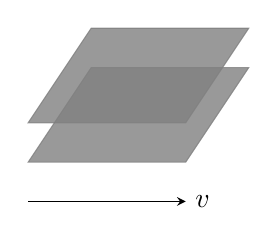
\begin{tikzpicture}
			\def\l{2};

			\begin{scope}[gray, opacity = 0.8]
				\filldraw (0,0) -- (\l,0) -- (\l + 0.4*\l, 0.6*\l) -- (0.4*\l, 0.6*\l) -- cycle;
				\filldraw[yshift = 0.5cm] (0,0) -- (\l,0) -- (\l + 0.4*\l, 0.6*\l) -- (0.4*\l, 0.6*\l) -- cycle;
			\end{scope}

			\draw[-stealth, yshift = -0.5cm] (0,0) -- (\l,0) node [right] {$v$};
		\end{tikzpicture}
	\end{figure}
	\begin{enumerate}
		\item Find the magnetic field between the plates and also above and below them.
		\item Find the magnetic force per unit area on the upper plate, including its direction.
		\item At what speed $v$ would the magnetic force balance the electric force?
	\end{enumerate}
\end{question}

\begin{solution}
	\begin{enumerate}[leftmargin = *]
		\item
			\begin{align*}
				I            & = k l        \\
                                             & = \sigma v l \\
				\therefore k & = \sigma v
			\end{align*}
			\begin{align*}
				B_{\textnormal{plate}} & = \frac{\mu_0 k}{2} \\
                                                       & = \frac{\mu_0 \sigma v}{2}
			\end{align*}
			By the right hand thumb rule, the magnetic field due to the upper plate is directed outwards for any point above it, and inwards for any point below it.\\
			Similarly, the magnetic field due to the lower plate is directed inwards for any point above it and outwards for any point below it.\\
			Therefore, for any point above the upper plate, and for any point below the lower plate, the magnetic field is cancelled out.
			Hence the net magnetic field above and below the plates is zero.\\
			At any point between the plates, the field adds up.\\
			Therefore,
			\begin{align*}
				B & = \frac{\mu_0 \sigma v}{2} + \frac{\mu_0 \sigma v}{2} \\
                                  & = \mu_0 \sigma v
			\end{align*}
			The field between the plates is directed inwards.
		\item
			\begin{align*}
				\overrightarrow{F}     & = q \overrightarrow{v} \times \overrightarrow{B}        \\
                                                       & = \sigma A \overrightarrow{v} \times \overrightarrow{B} \\
				\therefore F           & = \sigma A v B                                          \\
                                                       & = \sigma A v \frac{\mu_0 \sigma v}{2}                   \\
				\therefore \frac{F}{A} & = \frac{\mu_0 \sigma^2 v^2}{2}
			\end{align*}
			As $\overrightarrow{v}$ is directed to the right and $\overrightarrow{B}$ is directed inwards, $\overrightarrow{v} \times \overrightarrow{B}$ is directed upwards.\\
			Therefore, the force on the upper plate is directed upwards.
		\item
			The electric force acting on the upper plate due to the lower plate is
			\begin{align*}
				F_E & = \frac{\sigma^2}{2 \varepsilon_0} A
			\end{align*}
			The force is directed downwards.\\
			The magnetic force acting on the upper plate due to the lower plate is
			\begin{align*}
				F_B & = \frac{\mu_0 \sigma^2 v^2}{2} A
			\end{align*}
			The force is directed upwards.\\
			Therefore, if the forces are balanced,
			\begin{align*}
				F_E                                           & = F_B                            \\
				\therefore \frac{\sigma^2}{2 \varepsilon_0} A & = \frac{\mu_0 \sigma^2 v^2}{2} A \\
				\therefore \frac{1}{\varepsilon_0}            & = \mu_0 v^2                      \\
				\therefore v^2                                & = \frac{1}{\varepsilon_0 \mu_0}  \\
				\therefore v                                  & = \frac{1}{\sqrt{\varepsilon_0 \mu_0}}
			\end{align*}
	\end{enumerate}
\end{solution}

\end{document}
